\documentclass[a4paper,11pt]{article}
% Packages de base
\usepackage[utf8]{inputenc}
\usepackage[french]{babel}
\usepackage[T1]{fontenc}

\usepackage{graphicx}
\usepackage{float}
\usepackage{subfigure}

% Marges standard
\usepackage[top=2.5cm, bottom=2.5cm, left=2.5cm, right=2.5cm]{geometry}

% Pour avoir du code
\usepackage{listings}
\usepackage[usenames,dvipsnames]{color}    
 \lstset{ 
  language=R,                     % the language of the code
  basicstyle=\normalsize\ttfamily, % the size of the fonts that are used for the code
  numbers=left,                   % where to put the line-numbers
  numberstyle=\tiny\color{Blue},  % the style that is used for the line-numbers
  stepnumber=1,                   % the step between two line-numbers. If it is 1, each line
                                  % will be numbered
  numbersep=5pt,                  % how far the line-numbers are from the code
  backgroundcolor=\color{white},  % choose the background color. You must add \usepackage{color}
  showspaces=false,               % show spaces adding particular underscores
  showstringspaces=false,         % underline spaces within strings
  showtabs=false,                 % show tabs within strings adding particular underscores
  frame=single,                   % adds a frame around the code
  rulecolor=\color{black},        % if not set, the frame-color may be changed on line-breaks within not-black text (e.g. commens (green here))
  tabsize=2,                      % sets default tabsize to 2 spaces
  captionpos=b,                   % sets the caption-position to bottom
  breaklines=true,                % sets automatic line breaking
  breakatwhitespace=false,        % sets if automatic breaks should only happen at whitespace
  keywordstyle=\color{RoyalBlue},      % keyword style
  commentstyle=\color{ForestGreen},   % comment style
  stringstyle=\color{ForestGreen},      % string literal style
 literate={è}{{\`e}}1 {à}{{\`a}}1 {é}{{\'e}}1
} 


% Pour avoir les signets dans le PDF
\usepackage[hidelinks]{hyperref}
\usepackage{fancyhdr}
\usepackage{lastpage}
\pagestyle{fancy}
\fancyhf{}
 
\rfoot{Page \thepage \hspace{1pt}/\pageref{LastPage}}

% Pour faire des retours à la ligne dans les tableaux
\usepackage{tabularx}

% Titre
\title{Rapport Projet industriel : Prédiction de durées de séjours aux Hospices Civils de Lyon (HCL)}
\author{Grégoire MASSOT}
\date{25 Janvier 2016}

%Corps du document
\begin{document}
\sffamily
\maketitle
\begin{figure}[H]
\centering
\subfigure{
\includegraphics[height=4cm]{HCL.jpg}}
\subfigure{
\includegraphics[height=4cm]{Logo_emse.png}}
\end{figure}

\tableofcontents

\newpage

\section{Présentation du projet}
\subsection{Contexte du projet}
Ce projet industriel est orienté Data Science. Il s'agit de prédire le plus précisément possible des durées de séjour en milieu hospitalier à partir des données relatives aux patients à leur entrée à l'hôpital et des statistiques sur les patients précédents. Il s'agit donc d'un exercice d'apprentissage supervisé.
\newline
\newline
Ce projet s'inscrit dans une volonté de réduction des couts des Hopitaux Civils de Lyon (HCL). Une maximisation de l'occupation des lits hospitaliers permet d'accueillir plus de patients avec les moyens disponibles.
\subsection{Outils utilisés pour le projet}
On utilise exclusivement R et son interface Rstudio pour établir les prédictions. On utilisera les bibliothèques utiles pour le problème, en particulier \textbf{xgboost}

On utilisera LaTeX pour écrire les rapports (comme celui-ci). On utilise Antidote pour la correction orthographique.
\subsection{Présentation de la base de données}
On travaille sur la base de données hospitalière \texttt{base\_ano.txt} ayant le squelette suivant :

\begin{center}
\begin{tabular}{|c|c|c|c|c|}
\hline
\textbf{Duree du séjour} & Âge du patient & Diagnostic principal & Service hospitalier & ...\\
\hline
\textbf{duree1} & age1 & dp1 & service1 & ... \\
\hline
\textbf{duree2} & age2 & dp2 & service2 & ... \\
\hline
\textbf{duree3} & age3 & dp3 & service3 & ... \\
\hline
\textbf{...} & ... & ...  & ... & ...\\
\hline
\end{tabular}
\end{center}

La table contient les prédicteurs suivants :
\begin{center}
\begin{tabularx}{\textwidth}{|c|c|X|X|X|X|}
\hline
\textbf{Prédicteur} & Nature & Decription  & Modèle 1 & Modèle 2 & Modèle 3 \\
\hline
\textbf{moisent} & Discret & Numéro du mois lors de l'entrée du patient & Non & Oui & Oui \\
\hline
\textbf{moissor} & Discret & Numéro du mois lors de la sortie du patient & Non & Non & Non\\
\hline
\textbf{age} & Continu & Age du patient, en années & Oui & Oui & Oui\\
\hline
\textbf{codepos} & Discret & Code postal du domicile du patient  & Non & Oui & Oui \\
\hline
\textbf{MI-DEPR2} & Discrets & Comorbidités diagnostiquées & Non & Non & Oui \\
\hline
\textbf{Elix} & Discret & Nombre de comorbidités diagnostiquées & Non & Non & Oui \\
\hline
\textbf{centre} & Discret & Numéro du centre des HCL ou le patient a été pris en charge & Non & Oui & Oui\\
\hline
\textbf{service} & Discret & Numéro de l'unité médicale des HCL ou le patient a été pris en charge & Oui & Oui & Oui \\
\hline
\textbf{entree} & Discret & Mode d'entrée du patient & Non & Oui & Oui \\
\hline
\textbf{sortie} & Discret & Mode de sortie du patient & Non & Non & Non\\
\hline
\textbf{diag} & Discret & Diagnostic du patient selon la classification CIM-10 & Oui & Oui & Oui\\
\hline
\textbf{ID} & Discret & ID du séjour & Non & Non & Oui \\
\hline
\end{tabularx}
\end{center}

Dans le premier modèle, on garde seulement les prédicteurs de l'étude précédente. Dans le second modèle, on ajoute tous les prédicteurs qui sont connus de façon certaine lors de l'arrivée du patient.
\newline
\newline
Dans le dernier troisième modèle, on ajoute :
\begin{itemize}
\item Les comorbidités : elles ne sont pas connues de façon certaine lors de l'arrivée du patient
\item l'ID : Il permet de situer temporellement  le séjour par rapport aux autres dans la table. Ce n'est pas un prédicteur utilisable en pratique. Il permet cependant de mesurer l'importance de pouvoir situer les séjours dans le temps.
\end{itemize}
Le mois de sortie et le mode de sortie sont évidemment déterminés le jour de sortie du patient. On élimine donc ces données de la table pour tous les modèles.

\subsection{Chargement de la BDD}
On garde seulement les séjours dont la durée est supérieure ou égale à 1 jour. On découpe le jeu de données \texttt{donnees\_hcl} en un \texttt{TrainData} sur lequel on construira le modèle et un \texttt{TestData} sur lequel on comparera les durées de séjours prédites et les durées de séjour réelles.
\begin{lstlisting}
# Chargement de la BDD
donnees_hcl <- read.csv2(file = "base_ano.txt",header = TRUE, sep="\t")
# Sélection des variables (code à modifier en fonction du modèle)
donnees_hcl <- donnees_hcl[donnees_hcl$duree >= 1,]
donnees_hcl <- donnees_hcl[,-seq(8,57)]
donnees_hcl <- subset(donnees_hcl, select = -c(moissor, sortie))

# Transformation du facteur "age" en variable continue
donnees_hcl$age <- as.character(donnees_hcl$age)
donnees_hcl$age <- as.numeric(donnees_hcl$age)

# Création des jeux de Train et de Test
TrainData <- donnees_hcl[donnees_hcl$Selected == 1,]
TestData <- donnees_hcl[donnees_hcl$Selected == 0,]

predicteurs_Train <- subset(TrainData, select = -c(duree))
duree_Train <- subset(TrainData, select = c(duree))

predicteurs_Test <- subset(TestData, select = -c(duree))
duree_Test <- subset(TestData, select = c(duree))
\end{lstlisting}
\subsection{Mesure de la performance des modèles}
On utilisera le critère RMSE (\textit{Root Mean Square Error}) pour pouvoir mesurer la performance des modèles proposés. C'est le critère qui a été utilisé dans l'étude précédente. Cela permettra de mesurer la performance de cette étude.
\[
RMSE = \sqrt{\frac{1}{n}\sum_{i=1}^{n}(y_{i}-y_{i}^{pred})^{2}}
\]
\begin{lstlisting}
RMSE <- function(y, pred)
{
  sqrt(mean((y - pred)^2))
}
\end{lstlisting}

On utilise aussi le critère MAE (\textit{Mean Absolute Error}), plus parlant que le RMSE. C'est l'erreur moyenne sur les prévisions des durées de séjours (en jours)

\[
MAE = \frac{1}{n}\sum_{i=1}^{n}|y_{i}-y_{i}^{pred}|
\]

\begin{lstlisting}
MAE <- function(y, pred)
{
  mean(abs(y - pred))
}
\end{lstlisting}

\section{Modélisation du problème}
\subsection{Présentation de la méthode}
Le Gradient Boosting est une méthode de machine learning parmi les plus fréquemment utilisées pour les problèmes d'apprentissage supervisés. La bibliothèque xgboost est souvent utilisée dans les solutions gagnantes des challenges kaggle.
\subsection{Implémentation de la méthode}
\subsubsection{Réglage des paramètres}
Plusieurs paramètres sont à ajuster pour la méthode du gradient boosting. Les plus importants sont les suivants : 
\begin{itemize}
\item \texttt{nrounds} : c'est le nombre d'arbres à construire. Plus il est grand, plus la prédiction est exacte et plus le temps de simulation est long
\item \texttt{maxdepth} : c'est la profondeur maximale des arbres de décision.
\item \texttt{eta} : permet de régler le compromis biais/variance lors de l'apprentissage.
\end{itemize}
On utilise la fonction \texttt{train} du package \texttt{caret} pour pouvoir choisir au mieux ces paramètres.
\begin{lstlisting}
# Tuning des paramètres de xgboost
library(caret)
library(foreach)
library(doParallel)
cl <- makeCluster(8)

tuneGrid <- expand.grid(max_depth = c(2,4,6,8,10),
                        nrounds = 100,
                        eta = c(0.01,0.1,0.5,1))

fitControl <- trainControl(method = "repeatedcv",
                           number = 3,
                           repeats = 1)

xvalXGB <- train(TrainData$duree ~ .,
                 data = TrainData,
                 method = "xgbTree",
                 tuneGrid = tuneGrid,
                 trControl = fitControl)
\end{lstlisting}
\subsubsection{Construction du modèle}
Une fois ce réglage effectué, on peut lancer le gradient boosting sur le \texttt{TrainData} avec un nombre d'arbres le plus grand possible pour avoir le modèle le plus précis construit dans un temps raisonnable.
\begin{lstlisting}
# Construction du modèle
library(xgboost)
param <- list("objective" = "reg:linear",
              "eta"=0.5,
              "max.depth"=4,
              "nthread" = 8)

modelXgboost <- xgboost(data = as.matrix(predicteurs_Train)
                        , label = as.matrix(duree_Train)
                        , params=param
                        , nrounds = 100)
predictionXGBoost <- predict(modelXgboost,
                             as.matrix(predicteurs_Test))

RMSE(duree_Test, predictionXGBoost)
\end{lstlisting}

\section{Analyse des résultats}
\subsection{Importance des différentes variables}
On utilise l'outil \texttt{xgb.importance} fourni avec \texttt{xgboost} pour déterminer les prédicteurs retenus par l'algorithme de machine learning.

\begin{lstlisting}
names <- dimnames(predicteurs_Train)[[2]]
importance_matrix <- xgb.importance(names, model = modelXgboost)
xgb.plot.importance(importance_matrix)
xgb.plot.tree(feature_names = names, model = modelXgboost, n_first_tree = 2)
\end{lstlisting}

\subsubsection{1er Modèle}
\begin{figure}[H]
\begin{center}
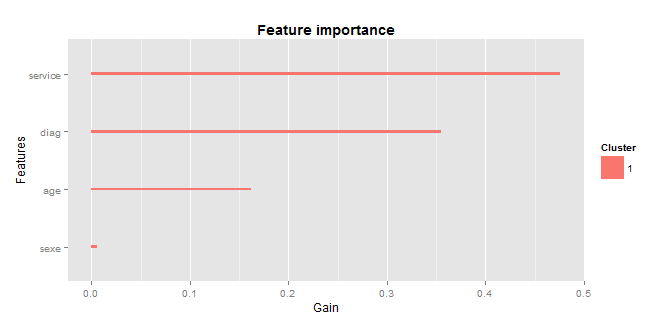
\includegraphics [width =18cm]{M1.png}
\end{center}
\end{figure}
\subsubsection{2nd Modèle}

\begin{figure}[H]
\begin{center}
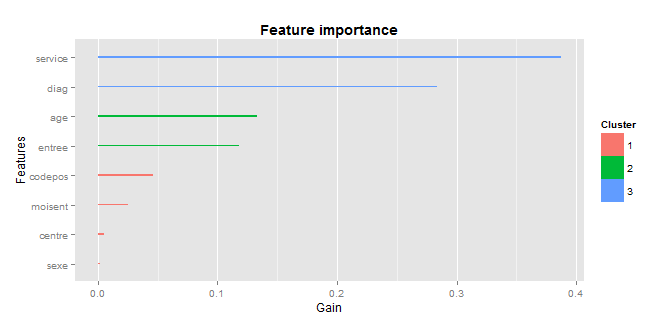
\includegraphics [width =18cm]{M2.png}
\end{center}
\end{figure}

\subsubsection{3ème Modèle}

\begin{figure}[H]
\begin{center}
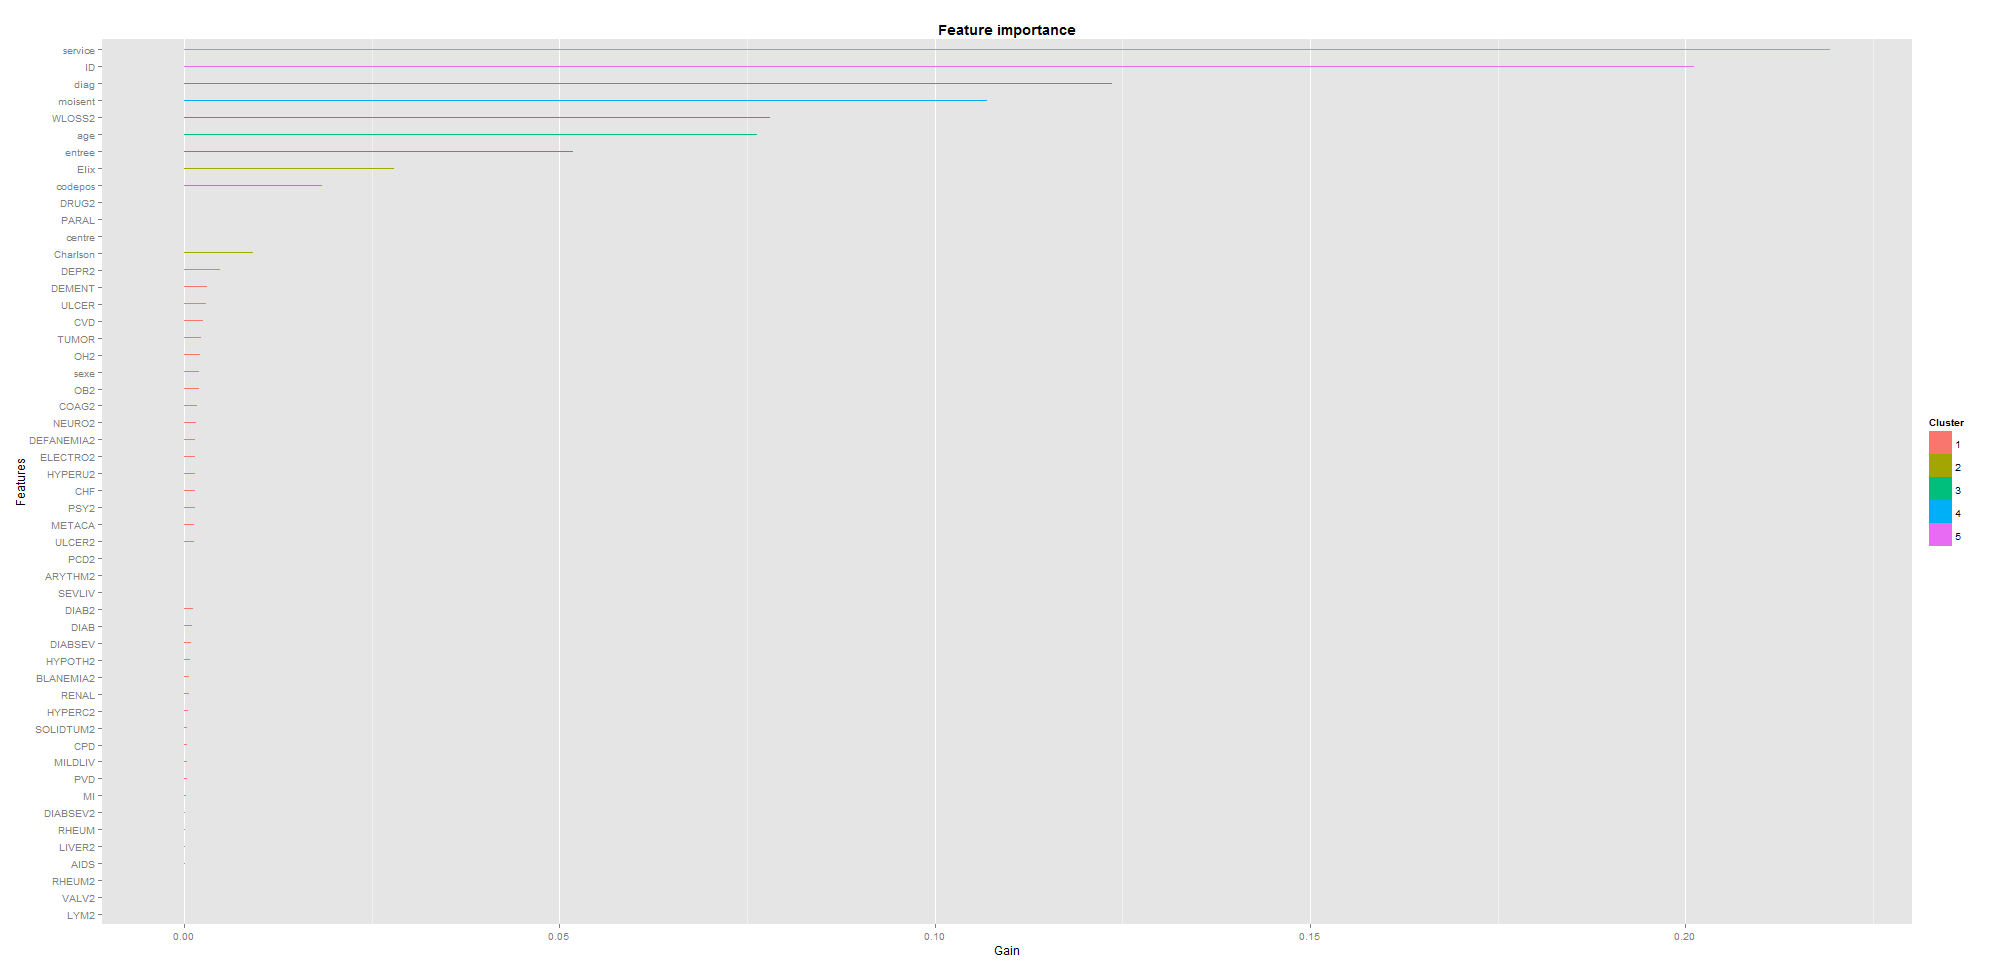
\includegraphics [width =18cm]{M3.png}
\end{center}
\end{figure}

\subsection{Performance des modèles}

\begin{center}
\begin{tabular}{|c|c|c|}
\hline
 & RMSE & MAE \\
\hline
Modèle 1 & 6.88 & 3.14 jours \\
\hline
Modèle 2 & 6.84 & 3.15 jours \\
\hline
Modèle 3 & 5.68 & 2.75 jours \\
\hline
\end{tabular}
\end{center}

On voit que l'ajout de l'identifiant (qui permet de situer le séjour temporellement par rapport aux autres) ainsi que certaines comorbidités permettent de gagner environ 10\% de MAE

\subsection{Incertitudes sur les résultats}

Pour améliorer la précision de la prédiction, on peut demander à xgboost de donner prédire non plus une durée brute, mais la densité de probabilité de la variable aléatoire relative à la durée de séjour.

Pour cela, on ajoute le code suivant lors du chargement des données

\begin{lstlisting}
donnees_hcl <- donnees_hcl[donnees_hcl$duree >= 1 & donnees_hcl$duree <= 30 ,]
duree_Test_RMSE <- subset(donnees_hcl[donnees_hcl$Selected == 0,], select = c(duree))
donnees_hcl$duree <- as.factor(donnees_hcl$duree)
\end{lstlisting}

On remplace aussi les paramètres de xgboost.

\begin{lstlisting}
param <- list("objective" = "multi:softprob",
              "eta"=0.3,
              "max.depth"=5,
              "nthread" = 8,
              "num_class" = 31)

modelXgboost <- xgboost(data = as.matrix(predicteurs_Train)
                        , label = as.matrix(duree_Train)
                        , params=param
                        , nrounds = 100)
xgbtest <- xgb.DMatrix(data.matrix(predicteurs_Test), missing=NA)

xgbpred <- predict(modelXgboost, xgbtest)
probs <- t(matrix(xgbpred, nrow=31, ncol=length(xgbpred)/31))
\end{lstlisting}

On affiche ensuite les résultats, par exemple, les 100 premières entrées du jeu de test

\begin{lstlisting}
for(i in 1:100)
{
  plot(probs[i,], type='l')
  abline(v=as.numeric(duree_Test$duree[i])+1, col="red")
}
\end{lstlisting}
On obtient des figures de ce type :

\begin{figure}[H]
\begin{center}
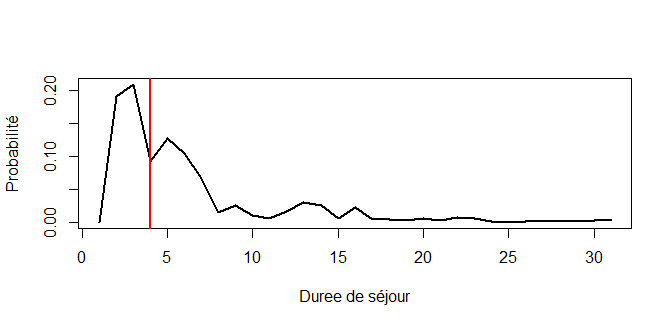
\includegraphics [width=12cm]{Densite.png}
\end{center}
\end{figure}

En noir la densité de probabilité de la variable aléatoire associée à la durée de séjour. En rouge la durée de séjour effectivement observée.

RMSE : 3.62
MAE : 2.24 jours

Les erreurs sont plus petites car on s'est limité aux séjours allant de moins de 30 jours afin de visualiser facilement les résultats sur un graphique.
\end{document}



